\noindent

\includegraphics[height=1.25cm]{images/pictograms/benchmark}

\includegraphics[height=1.25cm]{images/pictograms/under_construction}

\includegraphics[height=1.25cm]{images/pictograms/FEM}

\includegraphics[height=1.25cm]{images/pictograms/paraview}


%%%%%%%%%%%%%%%%%%%%%%%%%%%%%%%%%%%%%%%%%%%%%%%%%%%%%%%%%%%%%%%%%%%%%%%%%%%%%%%%%%%%%%%%%%%%%%%%%%%

\begin{flushright} {\tiny {\color{gray} python\_codes/fieldstone\_152/text.tex}} \end{flushright}

\lstinputlisting[language=bash,basicstyle=\small]{python_codes/fieldstone_152/keywords.key}

\par\noindent\rule{\textwidth}{0.4pt}

\begin{center}
\inpython
{\small Code: \url{https://github.com/cedrict/fieldstone/tree/master/python_codes/fieldstone_152}}
\end{center}

\par\noindent\rule{\textwidth}{0.4pt}

%{\sl This stone was developed in collaboration with Donald Duck}. \index{contributors}{D. Duck}

%\par\noindent\rule{\textwidth}{0.4pt}

%%%%%%%%%%%%%%%%%%%%%%%%%%%%%%%%%%%%%%%%%%%%%%%%%%%%%%%%%%%%%%%%%%%%%%%%%%%%%%%%%%%%%%%%%%%%%%%%%%%

The code for this \stone is based on \stone~\ref{f21}. 

The goal here is to explore the influence of the mapping polynomial order and/or
the number of quadrature points on the accuracy of the solution of the so-called 
annulus benchmark \ref{MMM-ss:sfan}.

We will explore:
\begin{itemize}
\item resolution {\python nelr=4-48}
\item {\python nqperdim=2,3,4,5}
\item {\python mapping='Q1','Q2','Q3','Q4'}
\end{itemize}
and will monitor the computed area, and the velocity and pressure errors.

After discretising the domain in {\python nel} elements, and having decided the FE
pair we want to use to solve the Stokes equations (in this case \QtwoQone), we end up 
having to compute elemental integrals such as 
\[
\K_e = \int_{\Omega_e} {\bm B}^T\cdot {\bm C} \cdot {\bm B} \; d\Omega
\]
The way we carry out integration is by means of the Gauss-Legendre quadrature, which 
forces us to carry out an change of variables from the original element $\Omega_e$ 
to the reference element $[-1,1]\times [-1,1]$. For this we establish a mapping between both 
as explained in Section~\ref{MMM-ss:mappings}.

\todo[inline]{
drawing of Q2Q1 nodes and mapping nodes Q1-Q4 next to them}


%%%%%%%%%%%%%%%%%%%%%%%%%%%%%%%
\section*{Areas and volumes}

Here we simply compute 
\[
{\cal A} = \sum_e \int_{\Omega_e} d\Omega
\]
where the sum runs over all elements of the annulus
and 
\[
{\cal V} = \sum_e \int_{\Omega_e} 2\pi x d\Omega
\]
for elements on the $x>0$ side of the annulus (axisymmetric formulation).
We of course have 
\[
{\cal A}_{analytical} = \pi (R_2^2-R_1^2)
\qquad\qquad
{\cal V}_{analytical} = \frac43 \pi (R_2^3-R_1^3)
\]
so that we can compute the relative errors as a function of resolution, mapping and quadrature: 
\begin{center}
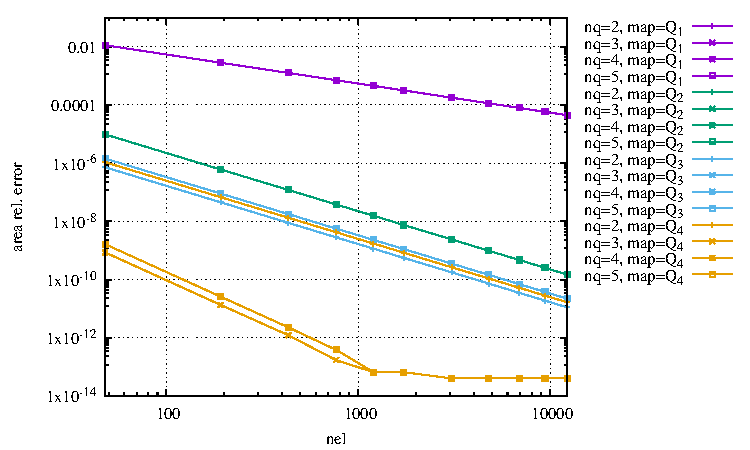
\includegraphics[width=8.3cm]{python_codes/fieldstone_152/results/areas/areas.pdf}
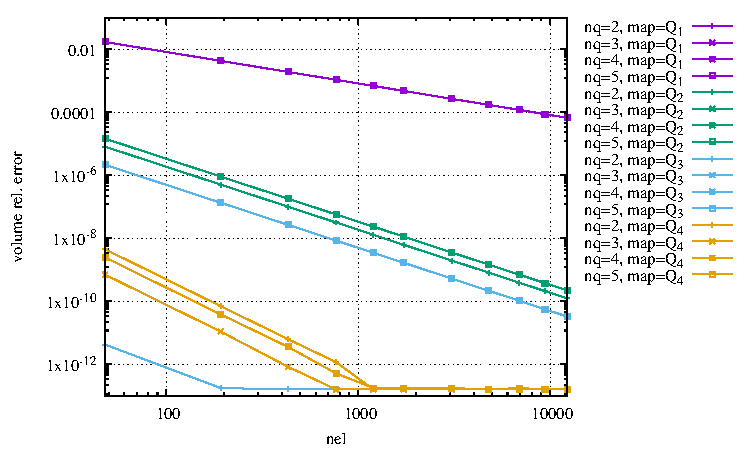
\includegraphics[width=8.3cm]{python_codes/fieldstone_152/results/areas/volumes.pdf}
\end{center}

Conclusions:
\begin{itemize}
\item unsurprisingly Q1 mapping yields the worst results
\item the type of mapping is the controling factor
\item for the isoparametric mapping $Q_2$ the number of quadrature points 
is not critical. Results are virtually identical for nqperdim=2,3,4,5
\item Q3 about one order of magnitude more accurate than Q2 
\item Q4 mapping 3-4 orders of magnitude more accurate than Q2 mapping
\item I can't explain the nqperdim=2/mapping=Q3 results that outperform everything else... (volume only)
\end{itemize}

Do these results translate to the solution of the Stokes system? Let's investigate...

%%%%%%%%%%%%%%%%%%%%%%%%%%%%%%%%%%%%%%%
\section*{Velocity and pressure errors}











%%%%%%%%%%%%%%%%%%%%%%%%%%%%%%%%%%%%%%%%%%%%%%%%%%%%%%%%%%%%%%%%%%%%%%%%%%%%%%%%%%%%%%%%%%%%%%%%%%%
\par\noindent\rule{\textwidth}{0.4pt}

\vspace{.5cm}

\begin{center}
\fbox{\begin{minipage}{0.9\textwidth}
{\color{teal}To Do, open questions, future work?}
\begin{itemize}
\item do smthg
\end{itemize}
\end{minipage}}
\end{center}

%%%%%%%%%%%%%%%%%%%%%%%%%%%%%%%%%%%%%%%%%%%%%%%%%%%%%%%%%%%%%%%%%%%%%%%%%%%%%%%%%%%%%%%%%%%%%%%%%%%
\vspace{.5cm}

\Literature:\\
\fullcite{xxxxYY}


